%%%%%%%%%%%%%%%%%%%%%%%%%%%%%%%%%%%%%%%%%%%%%%%%%%%%%%%%%%%%%%%%%%%%
% Author: A. Herrera Poyatos, Nuria Rodríguez Barroso
% Tittle: Familias de distribuciones
% Capítulo sobre familias de distribuciones importantes.
%%%%%%%%%%%%%%%%%%%%%%%%%%%%%%%%%%%%%%%%%%%%%%%%%%%%%%%%%%%%%%%%%%%%%

%!TEX root = ../inference.tex
%!TEX language = es

\section{Familias de distribuciones}

\subsection{Distribuciones discretas}

    En esta sección se desarrollan varias de las distribuciones discretas más importantes de la estadística.

    \subsubsection{Distribución uniforme}
La distribución uniforme es una distribución de probabilidad que asume un número finito de valores con la misma probabilidad. Es fácil comprobar que la función masa de probabilidad es $f(x|n) = \frac{1}{n}$. Claramente $\sum^n_{i=1} \frac{1}{n} = 1$.

La función generatriz de momentos es fácil calcularla y viene definida por $\varphi_X(t) = \frac{e^t (1 - e^tN)}{N(1-e^t)}$. De ella podemos obtener su media y varianza las cuales quedan de la siguiente forma:

\begin{center}
	$E[X] = \frac{N+1}{2}$
	\\$Var(X) =  E[X^2] - (E[X])^2 =  \frac{(N+1)(N-1)}{12}$
\end{center}

\subsubsection{Distribución de Poisson}
Esta distribución expresa, a partir de una frecuencia de ocurrencia media, la probabilidad de que ocurra un determinado número de eventos durante cierto período de tiempo. La función de masa o probabilidad de la distribución de Poisson es $f(x| \lambda) = \frac{e^{-\lambda}{\lambda}^x}{x!}$. \\Claramente $\sum^n_{i=1}  \frac{e^{-\lambda}{\lambda}^x}{x!} = e^{-\lambda} \sum^n_{i=1}  \frac{{\lambda}^x}{x!}  = 1$.


La función generatriz de momentos de dicha distribución se calcula de la siguiente manera $\varphi_X(t) = \sum^n_{i=0} \frac{e^{tx}e^{-\lambda}{\lambda}^x}{x!} = e^{-\lambda} \sum^n_{i=0}   \frac{(e^{t}  \lambda)^x}{x!} =  e^{-\lambda}  e ^{e^{t} \lambda} = e ^{\lambda (e^t -1 )}$.

A partir de la función generatriz de momentos podemos fácilmente deducir la media y la varianza:
\begin{center}
	$E[X] = \lambda $
	\\$Var(X) =  E[X^2] - (E[X])^2 =  \lambda$
\end{center}

\subsubsection{Distribución binomial}

Considérese un experimento de Bernoulli con probabilidad $\theta \in [0,1]$. Repetimos el experimento $n$ veces y nos preguntamos cuál es la probabilidad de que se hayan conseguido $x$ aciertos, donde $x = 0, 1, \ldots, n$. Es fácil ver que esta probabilidad viene dada por $\binom{n}{x} \theta^x (1-\theta)^{n-x}$. Esta cuestión, que es habitual en la estadística, origina la distribución binomial.

\begin{definition}
    Una variable aleatoria sigue una distribución binomial con parámetros $n \in \mathbb{N}$ y $\theta \in [0,1]$  si su función masa de probabilidad viene dada por $f(x|n,\theta) = \binom{n}{x} \theta^x (1-\theta)^{n-x}$. En tal caso se denota $X \sim B(x|n,\theta)$.
\end{definition}

\subsubsection{Distribución multinomial}

\begin{definition}
	La distribución multinomial se puede ver como una generalización de la distribución binomial para variables politómicas (variables discretas con más de dos categorías).
	\\Supongamos que se realizan $n$ ensayos independientes que dan lugar a $k$ resultados distintos $X = (X_1, ... X_k)$  con probabilidades $\theta_1, ... , \theta_k$ respectivamente, donde $\theta_1+... + \theta_k = 1$. Entonces, la función de probabilidad para dicha variable multinomial sería:

	\[
	f(X|\theta_1, ... , \theta_k) = \frac{n!}{X_1! X_2! ... X_k!} \theta^{X_1} \theta^{X_2} ... \theta^{X_k}
	\]

\end{definition}


\subsection{Distribuciones continuas}

En esta sección se desarrollan varias de las distribuciones continuas más importantes de la estadística.

\subsubsection{Distribución uniforme}

La distribución uniforme asigna una credibilidad uniforme a todos los puntos de un intervalo $[a,b]$. Esto es, su función de densidad viene dada por
\[f(x|a,b) = \begin{cases}\frac{1}{b-a} \text{ si } x \in [a,b], \\ 0 \text{ en otro caso.}\end{cases}\]
Claramente tenemos que $\int_{-\infty}^{\infty} f(x |a,b) dx = 1$. Además, podemos calcular fácilmente sus momentos como sigue (y, por tanto, también su varianza)
\[E[X^j] = \int_a^b \frac{x^j}{b-a} dx = \frac{b^{j+1} - a^{j+1}}{(b-a) (j+1)},\]
\[Var(X) = E[X^2] - E[X]^2 = \frac{a^2 + ab + b^2}{3} - \frac{(a+b^2)}{4} = \frac{(b-a)^2}{12}.\]

\subsubsection{Distribución normal}

La distribución normal, también llamada distribución gaussiana, es la distribución más importante de la estadística. Esto se debe a sus numerosas aplicaciones en análisis de poblaciones y al teorema central del límite.

\begin{definition}
    Sean $\mu \in \mathbb{R}$ y $\sigma^2 > 0$. Definimos la distribución $N(x | \mu, \sigma^2)$ como la distribución que tiene función de densidad
    \[f(x | \mu, \sigma^2) = \frac{1}{\sqrt{2\pi}\sigma}e^{-(x-\mu)^2 / (2\sigma^2)}, x \in \mathbb{R}.\]
\end{definition}

La distribución normal está bien definida como consecuencia del siguiente lema.
\begin{lem}
    Sean $\mu \in \mathbb{R}$ y $\sigma > 0$. Tenemos que $\int_{-\infty}^\infty e^{-(x-\mu)^2 / (2\sigma^2)}dx = \sqrt{2\pi}\sigma.$
\end{lem}
\begin{proof}
    En primer lugar, vamos a calcular la integral para $\mu = 0$ y $\sigma = 1$. La demostración consiste en reducir el problema en calcular una integral en dos variables. Para ello, elevamos al cuadrado y obtenemos
    \[\left(\int_{-\infty}^\infty e^{-x^2 / 2}dx\right)^2 = \left(\int_{-\infty}^\infty e^{-t^2 / 2}dt\right) \left(\int_{-\infty}^\infty e^{-s^2 / 2}ds \right) = \int_{-\infty}^\infty \int_{-\infty}^\infty e^{-(t^2+s^2) / 2} dt ds. \]
    Resolvemos esta última integral mediante un cambio a polares
    \[\int_{-\infty}^\infty \int_{-\infty}^\infty e^{-(t^2+s^2) / 2} dt ds = \int_{-\pi}^\pi \left(\int_{0}^\infty \rho e^{-\rho^2 / 2} d\rho \right) d\theta = 2\pi \int_{0}^\infty \rho e^{-\rho^2 / 2} d\rho = 2\pi.\]
    Por último, utilizamos el cambio de variable $y = (x - \mu) / \sigma$ para obtener
    \[\int_{-\infty}^\infty e^{-(x-\mu)^2 / (2\sigma^2)}dx = \int_{-\infty}^\infty \sigma e^{-y^2 / 2}dy = \sqrt{2\pi}\sigma. \qedhere\]
\end{proof}

Nótese que si $X \sim N(x | \mu, \sigma^2)$, entonces $Y = (X - \mu)/\sigma$ sigue una distribución $N(x|0,1)$.

\begin{prop} \label{prop:normal:cf}
    La función característica de la distribución $N(x|\mu, \sigma^2)$ viene dada por $\varphi_X(t) = e^{it\mu - t^2 \sigma^2 / 2}$.
\end{prop}
\begin{proof}
    En primer lugar, tenemos que
    \[\varphi_X(t) = E[e^{itX}] = \frac{1}{\sqrt{2\pi}\sigma} \int_{-\infty}^{\infty} e^{itx-(x-\mu)^2 / (2\sigma^2)} dx = \frac{1}{\sqrt{2\pi}\sigma} \int_{-\infty}^{\infty} e^{-((x-\mu)^2 - 2itx\sigma^2) / (2\sigma^2)} dx.\]
    Completamos cuadrados como sigue
    \[(x-\mu)^2 - 2 itx\sigma^2 = (x - (it \sigma^2 + \mu))^2 + t^2 \sigma^4 - 2it\sigma^2 \mu.\]
    Esto sugiere utilizar el cambio de variable $g(y) = y + it \sigma^2$. Obtenemos
    \begin{align*}
        \sqrt{2\pi}\sigma \varphi_X(t) = \int_{-\infty}^{\infty} e^{-((x-\mu)^2 - 2itx\sigma^2) / (2\sigma^2)} = e^{it\mu - t^2 \sigma^2 / 2} \int_{-\infty}^{\infty} e^{-((x-(it \sigma^2 + \mu))^2 ) / (2\sigma^2)} dx \\
        = e^{it\mu - t^2 \sigma^2 / 2} \int_{-\infty}^{\infty} e^{-(y - \mu)^2 ) / (2\sigma^2)} dy = \sqrt{2\pi}\sigma e^{it\mu - t^2 \sigma^2 / 2},
    \end{align*}
    como se quería.
    Nótese que a pesar de ser una integral de contorno compleja el cambio de variable es válido. En efecto, el cambio de variable es afín y la función a integrar es entera. Por tanto, utilizando el camino cerrado $g([0, \infty]) + [\infty, 0]$ se puede probar que el cambio es válido.
\end{proof}

Análogamente se puede probar el siguiente resultado.

\begin{prop} \label{prop:normal:gm}
    La función generatriz de momentos de la distribución $N(x|\mu, \sigma^2)$ viene dada por $\varphi_X(t) = e^{t\mu - t^2 \sigma^2 / 2}$.
\end{prop}

\begin{cor} \label{cor:normal:rec}
    Los momentos de la distribución $N(x|\mu,\sigma^2)$ verifican la ecuación recurrente
    \[E[X^k] = -(k-1)\sigma^2 E[X^{k-2}] + (\mu - t \sigma^2) E[X^{k-1}], \ \  k \ge 2.\]
\end{cor}
\begin{proof}
    Sabemos que $E[X^k] = \varphi_X^{(k)}(t)$. Tenemos $\varphi_X^{(1)}(t) = (\mu - t \sigma^2) \varphi_X(t)$. Consecuentemente,
    \[\varphi_X^{(2)}(t) = -\sigma^2 \varphi_X(t) + (\mu - t \sigma^2) \varphi_X^{(1)}(t).\]
    Por inducción se extiende el resultado fácilmente para $k \ge 2$.
\end{proof}

\begin{cor}
    Si $X \sim N(x|\mu,\sigma^2)$, entonces $E[X] = \mu$ y $E[X^2] = \sigma^2 + \mu^2$. Consecuentemente, $Var(X) = \sigma^2$. Como consecuencia de este resultado al parámetro $\mu$ se le llama media y al parámetro $\sigma^2$ varianza.
\end{cor}

Podemos utilizar los dos corolarios anteriores para calcular los momentos de la distribución normal resolviendo una ecuación recurrente de segundo orden. Evidentemente, la fórmula obtenida será bastante larga. Sin embargo, esta ecuación se simplifica en el caso de los momentos centrados, como pone de manifiesto el siguiente resultado, que se puede demostrar fácilmente por inducción a partir del Corolario \ref{cor:normal:rec}.

\begin{cor}
    Si $X \sim N(x|0,\sigma^2)$, entonces
    \[E[X^k] = \begin{cases} 0 & \text{ si } k \text{ es impar;} \\ (k-1)!! \sigma^{k} & \text{ si } k \text{ es par;} \end{cases}\]
    donde $n!!$ denota al doble factorial, definido como el producto de los números desde $1$ hasta $n$ con la misma paridad que $n$.
\end{cor}

La Figura \ref{fig:normal} muestra la función de densidad de una distribución normal. Podemos ver que la densidad se concentra en torno a la media. De hecho, $P(|X - \mu| \ge 2\sigma) \approx 0.046$. Es más, $P(|X - \mu| \ge 3\sigma) \approx 0.03$.

\begin{figure}[H]
\centering
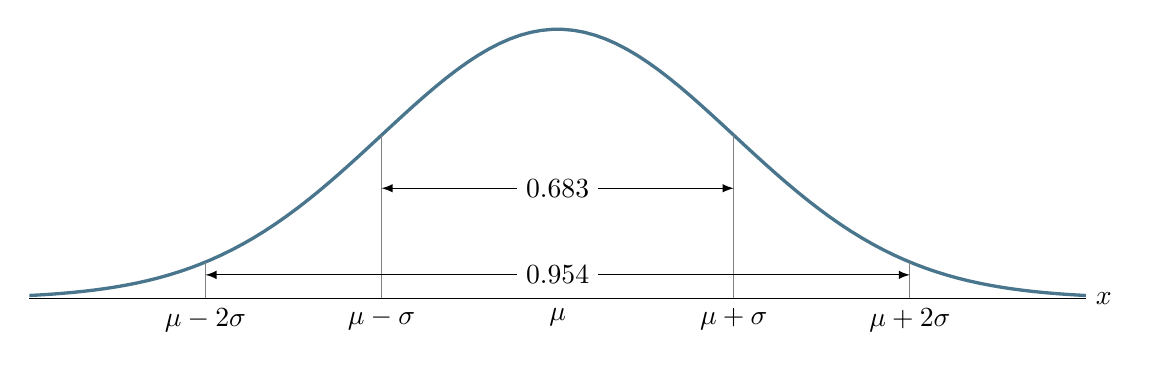
\begin{tikzpicture}[
     declare function={gauss(\x,\mu,\sigma)=1/(\sigma*sqrt(2*pi))*exp(-((\x-\mu)^2)/(2*\sigma^2));}
    ]
\begin{axis}[
    no markers,
    domain=0:6,
    samples=100,
    ymin=0,
    axis lines*=left,
    xlabel=$x$,
    every axis y label/.style={at=(current axis.above origin),anchor=south},
    every axis x label/.style={at=(current axis.right of origin),anchor=west},
    height=5cm,
    width=15cm,
    xtick=\empty,
    ytick=\empty,
    enlargelimits=false,
    clip=false,
    axis on top,
    grid = major,
    hide y axis
]

\addplot[very thick,cyan!50!black] {gauss(x, 3, 1)};

        \pgfmathsetmacro\valueA{gauss(1,3,1)}
        \pgfmathsetmacro\valueB{gauss(2,3,1)}
        \draw [gray] (axis cs:1,0) -- (axis cs:1,\valueA)
            (axis cs:5,0) -- (axis cs:5,\valueA);
            \draw [gray] (axis cs:2,0) -- (axis cs:2,\valueB)
            (axis cs:4,0) -- (axis cs:4,\valueB);
            \draw [yshift=1.4cm, latex-latex](axis cs:2, 0) -- node [fill=white] {$0.683$} (axis  cs:4, 0);
            \draw [yshift=0.3cm, latex-latex](axis cs:1, 0) -- node [fill=white] {$0.954$} (axis cs:5, 0);

            \node[below] at (axis cs:1, 0)  {$\mu - 2\sigma$};
            \node[below] at (axis cs:2, 0)  {$\mu - \sigma$};
            \node[below] at (axis cs:3, 0)  {$\mu$};
            \node[below] at (axis cs:4, 0)  {$\mu + \sigma$};
            \node[below] at (axis cs:5, 0)  {$\mu + 2\sigma$};
\end{axis}

\end{tikzpicture}
\caption{Función de densidad de una distribución normal.}
\label{fig:normal}
\end{figure}

\begin{prop}
    Sean $X_1$ e $Y_2$ dos variables aleatorias independientes que siguen una distribución $N(x|\mu_1,\sigma_1^2)$ y $N(x|\mu_2,\sigma_2^2)$ respectivamente. Entonces $X+Y$ sigue una distribución $N(x|\mu_1+\mu_2,\sigma_1^2+\sigma_2^2)$.
\end{prop}
\begin{proof}
    Basta darse cuenta de que $\varphi_{X+Y}(t) = \varphi_{X}(t)\varphi_{Y}(t) = e^{t(\mu_1 + \mu_2) - t^2 (\sigma_1^2 + \sigma_2^2) / 2}$ es la función característica asociada a la distribución $N(x|\mu_1+\mu_2,\sigma_1^2+\sigma_2^2)$. Recordemos que la función característica determina de forma unívoca a la distribución.
\end{proof}

El recíproco del resultado anterior también es cierto.

\begin{thm}[Cramer]
    Sean $X$ e $Y$ dos variables aleatorias independientes. Si $X+Y$ es normal, entonces $X$ e $Y$ son normales.
\end{thm}

\subsubsection{Distribución gamma}

La famila de distribuciones gamma se encuentra definida sobre el intervalo $[0, \infty)$. En su definición entra en juego la famosa función gamma, de ahí su nombre.

\begin{definition}
    Se define la función gamma como la aplicación $\Gamma: (0, \infty) \to (0, \infty)$ dada por
    \[\Gamma(\alpha) = \int_0^\infty t^{\alpha-1}e^{-t}dt.\]
\end{definition}
\begin{prop}
    La función gamma está bien definida.
\end{prop}
\begin{proof}
    Sea $\alpha > 0$. Tenemos que probar que $\int_0^\infty t^{\alpha-1}e^{-t}dt < \infty$. Tomando $b > 0$, escribimos
    \[\int_0^\infty t^{\alpha-1}e^{-t}dt = \int_0^b t^{\alpha-1}e^{-t}dt + \int_b^\infty t^{\alpha-1}e^{-t}dt.\]
    Sabemos que la función $t^{\alpha - 1}$ tiene a $t^{\alpha} / \alpha$ como primitiva y, por tanto, es integrable en $[0,b]$. Puesto que $t^{\alpha-1}e^{-t} \le t^{\alpha-1}$, obtenemos que $t^{\alpha-1}e^{-t}$ es integrable en $[0,b]$. Por otro lado tenemos que
    \[\lim_{t \to \infty} \frac{t^{\alpha-1}e^{-t}}{e^{-t / 2}} = 0.\]
    Consecuentemente, para cierto $b > 0$ se verifica $t^{\alpha-1}e^{-t} \le e^{-t / 2}$ para todo $t \ge b$. Puesto que $e^{-t / 2}$ es integrable en $[b, \infty)$, deducimos que $t^{\alpha-1}e^{-t}$ también lo es, lo que termina la demostración.
\end{proof}

\begin{prop}[Propiedades de la función gamma]
    Sea $\alpha > 0$. Se verifica:
    \begin{enumerate}
        \item $\Gamma(1) = 1$;
	\item $\Gamma(\alpha+1) = \alpha\Gamma(\alpha)$;
    \item $\Gamma(n+1) = n!$ para cualquier $n \in \mathbb{N}$;
    \item (Fórmula de reflexión de Euler) si $0 < \alpha < 1$, entonces $\Gamma(\alpha) \Gamma(1- \alpha) = \frac{\pi}{\sin(\alpha \pi)}$;
    \item $\Gamma(1/2) = \sqrt{\pi}$;
    \item $\Gamma(\alpha) = \beta^\alpha\int_0^\infty t^{\alpha-1}e^{-\beta t} dt$ para todo $\beta > 0$.
    \end{enumerate}
\end{prop}
\begin{proof}
    \
    \begin{enumerate}
        \item Es fácil ver que $\int_{0}^\infty e^{-t} dt = 1$.
        \item Integrando por partes obtemos
        \[\Gamma(\alpha+1) = \int_0^{\infty}{t^{\alpha}e^{-t}dt} = \bigg[-e^{-t}t^\alpha\bigg]_0^{\infty} +
            \int_0^{\infty}{xt^{\alpha-1}e^{-t}dt} = \alpha\int_0^{\infty}{t^{\alpha-1}e^{-t}dt} = \alpha\Gamma(\alpha).\]
        \item Es consecuencia directa de los apartados a) y b).
        \item Se obtiene utilizando definiciones alternativas de la función gamma tras extenderla a $\mathbb{C} \setminus \mathbb{Z}^-_0$. Para más información véase \cite{gamma}. No desarrollamos esta demostración pues solo la necesitamos para el siguiente apartado.
        \item Se obtiene al evaluar la fórmula de reflexión en $\alpha = 1/2$.
        \item Se obtiene realizando el cambio de variable $t = \beta s$. \qedhere
    \end{enumerate}
\end{proof}

\begin{definition}
    Sean $\alpha, \beta > 0$. Definimos la distribución $Gamma(x | \alpha, \beta)$ como la distribución que tiene función de densidad
    \[f(x | \alpha, \beta) = \frac{\beta^\alpha}{\Gamma(\alpha)}x^{\alpha-1}e^{-\beta x}, x > 0.\]
\end{definition}

El parámetro $\alpha$ se conoce como parámetro de forma ya que influencia la forma de la distribución, como muestra el siguiente resultado.

\begin{prop}
    La función de densidad de la distribución $Gamma(\alpha, \beta)$ verifica las siguientes propiedades:
    \begin{itemize}
        \item Si $0< \alpha <1$, entonces $f(x | \alpha, \beta)$ es decreciente y $f(x) \to \infty$ para $x \to 0$.
        \item Si $\alpha = 1$, entonces $f(x | \alpha, \beta)$ es decreciente con $f(0) = 1$.
        \item Si $\alpha > 1$, entonces $f(x | \alpha, \beta)$ crece en $[0, (\alpha-1) / \beta]$ y decrece en $[(\alpha-1) / \beta,\infty]$.
        \item Si $0 < \alpha \le 1$, entonces $f(x | \alpha, \beta)$ es convexa.
        \item Si $1 < \alpha \le 2$, entonces $f(x | \alpha, \beta)$ es cóncava en $[0,(\alpha-1 + \sqrt{\alpha - 1}) / \beta]$ y convexa en $[(\alpha-1 + \sqrt{\alpha - 1}) / \beta, \infty]$.
        \item Si $2 < \alpha$, entonces $f(x | \alpha, \beta)$ es cóncava en $[(\alpha-1 - \sqrt{\alpha - 1}) / \beta,(\alpha-1 + \sqrt{\alpha - 1}) / \beta]$ y convexa en $[0, (\alpha-1 - \sqrt{\alpha - 1}) / \beta]$ y $[(\alpha-1 + \sqrt{\alpha - 1}) / \beta, \infty]$.
    \end{itemize}
\end{prop}
\begin{proof}
Los resultados se obtienen mediante las herramientas habituales del cálculo. Basta estudiar la derivada primera y la derivada segunda
\begin{align*}
f^\prime(x) &= \frac{\beta^\alpha}{\Gamma(\alpha)} x^{\alpha-2} e^{-\beta x}[(\alpha - 1) - \beta x]; \\
f^{\prime \prime}(x) &= \frac{\beta^\alpha}{\Gamma(\alpha)} x^{\alpha-3} e^{-\beta x} \left[(\alpha - 1)(\alpha - 2) - 2 \beta (\alpha - 1) x + \beta^2 x^2\right]. \qedhere
\end{align*}
\end{proof}

La Figura \ref{fig:gamma:alpha} muestra la función de densidad de la distribución gamma para distintos valores de $\alpha$.  El parámetro $\beta$ se denomina parámetro de escala debido a su influencia en la escala de la función de densidad. La Figura \ref{fig:gamma:beta} muestra la función de densidad de la distribución gamma para distintos valores de $\beta$.

\begin{figure}[H]
    \centering
    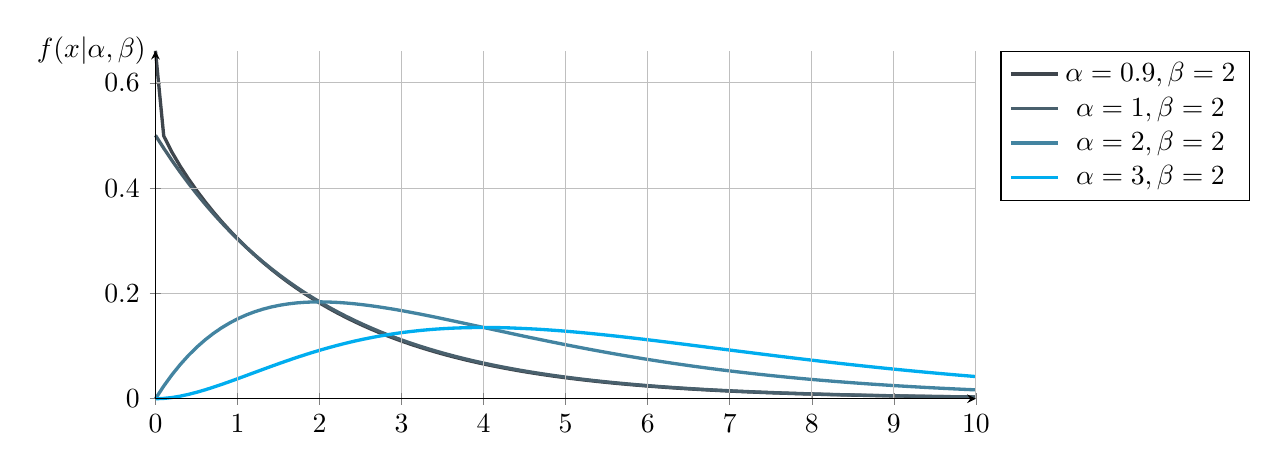
\begin{tikzpicture}[
        declare function={gamma(\z)=
        2.506628274631*sqrt(1/\z)+ 0.20888568*(1/\z)^(1.5)+ 0.00870357*(1/\z)^(2.5)- (174.2106599*(1/\z)^(3.5))/25920- (715.6423511*(1/\z)^(4.5))/1244160)*exp((-ln(1/\z)-1)*\z;},
        declare function={gammapdf(\x,\k,\theta) = 1/(\theta^\k)*1/(gamma(\k))*\x^(\k-1)*exp(-\x/\theta);}
        ]
        \begin{axis}[
            ylabel={$f(x | \alpha, \beta)$},
            domain=0.000001:10, samples=100,
            axis lines=left,
            every axis y label/.style={at=(current axis.above origin),anchor=east},
            every axis x label/.style={at=(current axis.right of origin),anchor=north},
            height=6cm, width=12cm,
            enlargelimits=false,
            clip=false,
            axis on top,
            grid = major,
            legend pos=outer north east
        ]
            \addplot [very thick,cyan!20!black] {gammapdf(x,0.98,2)};
            \addlegendentry{$\alpha = 0.9, \beta = 2$}
            \addplot [very thick,cyan!35!black] {gammapdf(x,1,2)};
            \addlegendentry{$\alpha = 1, \beta = 2$}
            \addplot [very thick,cyan!60!black] {gammapdf(x,2,2)};
            \addlegendentry{$\alpha = 2, \beta = 2$}
            \addplot [very thick,cyan] {gammapdf(x,3,2)};
            \addlegendentry{$\alpha = 3, \beta = 2$}
        \end{axis}
    \end{tikzpicture}
    \caption{Densidad de la distribución gamma con distintos valores de $\alpha$.}
    \label{fig:gamma:alpha}
\end{figure}

\begin{figure}[H]
    \centering
    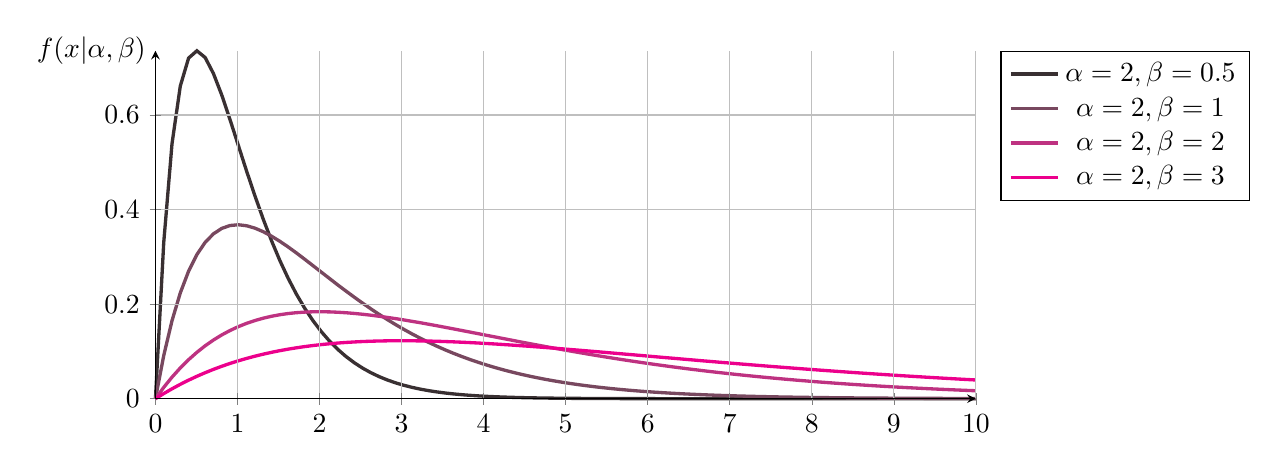
\begin{tikzpicture}[
        declare function={gamma(\z)=
        2.506628274631*sqrt(1/\z)+ 0.20888568*(1/\z)^(1.5)+ 0.00870357*(1/\z)^(2.5)- (174.2106599*(1/\z)^(3.5))/25920- (715.6423511*(1/\z)^(4.5))/1244160)*exp((-ln(1/\z)-1)*\z;},
        declare function={gammapdf(\x,\k,\theta) = 1/(\theta^\k)*1/(gamma(\k))*\x^(\k-1)*exp(-\x/\theta);}
        ]
        \begin{axis}[
            ylabel={$f(x | \alpha, \beta)$},
            domain=0:10, samples=100,
            axis lines=left,
            every axis y label/.style={at=(current axis.above origin),anchor=east},
            every axis x label/.style={at=(current axis.right of origin),anchor=north},
            height=6cm, width=12cm,
            enlargelimits=false, clip=false, axis on top,
            grid = major,
            legend pos=outer north east
        ]
            \addplot [very thick,magenta!10!black] {gammapdf(x,2,0.5)};
            \addlegendentry{$\alpha = 2, \beta = 0.5$}
            \addplot [very thick,magenta!40!black] {gammapdf(x,2,1)};
            \addlegendentry{$\alpha = 2, \beta = 1$}
            \addplot [very thick,magenta!75!black] {gammapdf(x,2,2)};
            \addlegendentry{$\alpha = 2, \beta = 2$}
            \addplot [very thick,magenta] {gammapdf(x,2,3)};
            \addlegendentry{$\alpha = 2, \beta = 3$}
        \end{axis}
    \end{tikzpicture}
    \caption{Densidad de la distribución gamma con distintos valores de $\beta$.}
    \label{fig:gamma:beta}
\end{figure}

\begin{prop} \label{prop:gamma:cf}
    La función característica de la distribución $Gamma(x|\alpha, \beta)$ viene dada por $\varphi_X(t) = \left(\frac{\beta}{\beta -it}\right)^\alpha$.
\end{prop}
\begin{proof}
    Basta utilizar el cambio de variable $g(y) = y / (\beta - it)$ como sigue
    \[E[e^{itX}] = \frac{\beta^\alpha}{\Gamma(\alpha)} \int_{0}^{\infty} x^{\alpha-1}e^{-(\beta - it) x} dx = \frac{\beta^\alpha}{\Gamma(\alpha) (\beta -it)^\alpha} \int_{0}^{\infty} y^{\alpha-1}e^{-y} dy = \left(\frac{\beta}{\beta -it}\right)^\alpha.\]
    Nótese que a pesar de ser una integral de contorno compleja el cambio de variable afín es válido como se comentó en la Proposición \ref{prop:normal:cf}.
\end{proof}

\begin{cor}
    El momento $k$-ésimo de la distribución $Gamma(x|\alpha,\beta)$ es $\alpha (\alpha+1) \ldots (\alpha + k -1) / \beta^k$.
\end{cor}
\begin{proof}
    Tenemos que $i^k E[X^k]= \varphi_X^{(k)}(t) = i^k \alpha (\alpha+1) \ldots (\alpha + k -1) / \beta^k$.
\end{proof}

\begin{prop}
    La función generatriz de momentos de la distribución $Gamma(x|\alpha, \beta)$ viene dada por $\varphi_X(t) = \left(\frac{\beta}{\beta - t}\right)^\alpha$.
\end{prop}
\begin{proof}
    La demostración es análoga a la dada en la Proposición \ref{prop:gamma:cf}.
\end{proof}

\begin{cor}
    La distribución $Gamma(x|\alpha,\beta)$ tiene media $\alpha / \beta$ y varianza $\alpha / \beta^2$.
\end{cor}

\begin{prop}
    Sea $n \ge 1$. Consideremos $X_1, \ldots, X_n$ variables aleatorias independientes tales que $X_j$ sigue una distribución $Gamma(x|\alpha_i, \beta)$. Entonces, $\sum_{i=1}^n X_j$ sigue una distribución $Gamma(x|\sum_{i=1}^n \alpha_i, \beta)$.
\end{prop}
\begin{proof}
    En primer lugar, calculamos la función característica de $\sum_{i=1}^n X_j$ como sigue
    \[E[e^{i\sum X_j}] = E[\prod e^{iX_j}] = \prod E[e^{iX_j}] = \left(\frac{\beta}{\beta - it}\right)^{\sum \alpha_j},\]
    donde se ha utilizado que la esperanza del producto de dos variables aleatorias independientes es el producto de las esperanzas. Por último, nótese que la función característica de la variable $\sum X_j$ es la función característica de $Gamma(x|\sum_{i=1}^n \alpha_i, \beta)$. El hecho de que la función característica de una distribución la determina de forma unívoca finaliza la prueba.
\end{proof}

\begin{prop} \label{prop:normal-square}
    Sea $X \sim N(x|0,\sigma^2)$. La variable aleatoria $Y = X^2$ sigue una distribución \\ $Gamma(y,1/2,1/(2\sigma^2))$. En particular, para $\sigma = 1$, $Y = X^2$ sigue una distribución $\chi^2_1$.
\end{prop}
\begin{proof}
    Sean $F$ y $G$ las funciones de distribución de las variables $X$ e $Y$ respectivamente. Tenemos que $G(y) = P(X^2 \le y) = P(- \sqrt{y} \le X \le \sqrt{y}) = F(\sqrt{y}) - F(-\sqrt{y})$. Derivando, obtenemos
    \[G'(y) = \frac{F'(\sqrt{y}) + F'(-\sqrt{y})}{2\sqrt{y}} = \frac{1}{\sqrt{y}} \frac{1}{\sqrt{2\pi}\sigma} e^{-y/(2\sigma^2)} = \frac{(1/(2\sigma^2))^{1/2}}{\Gamma(1/2)} y^{-1/2} e^{-y/(2\sigma^2)}.\]
    Por último, basta darse cuenta de que $G'(y)$ es la función de densidad de $Gamma(y,1/2,1/(2\sigma^2))$.
\end{proof}

\subsubsection{Distribución beta}

La famila de distribuciones beta se encuentra definida sobre el intervalo $(0, 1)$. En su definición entra en juego la denominada función beta, de ahí su nombre.

\begin{definition}
    Se define la función beta como la aplicación $\beta : (0, \infty) \times (0, \infty) \to (0, \infty)$ dada por
    \[\beta(x, y) = \int_0^1 t^{x-1}(1-t)^{y-1}\,dt.\]
\end{definition}
\begin{prop} \label{prop:beta-gamma}
    Para cada $x, y > 0$ se tiene que $\frac{\Gamma(x)\Gamma(y)}{\Gamma(x+y)} = \beta(x,y)$. Como consecuencia, la función beta está bien definida.
\end{prop}
\begin{proof}
    En primer lugar escribimos $\Gamma(x)\Gamma(y)$ como una integral doble
    \begin{equation*}
        \Gamma(x)\Gamma(y) =\int_{0}^{\infty }\ e^{-u}u^{x-1}\,d u\int_{0}^{\infty }\ e^{-v}v^{y-1}\,d v
        =\int_{0}^{\infty }\int_{0}^{\infty }\ e^{-u-v}u^{x-1}v^{y-1}\,d u\,d v.
    \end{equation*}
    La expresión anterior nos sugiere utilizar el cambio de variable $(u, v) = J(t,s) = (st, (1-t)s)$. Nótese que $|J(t,s)| = s$. Aplicamos el cambio a continuación
    \begin{gather*}
        \Gamma(x)\Gamma(y) = \int_{0}^{\infty} \left( \int_{0}^{1}e^{-s}(st)^{x-1}(s(1-t))^{y-1}|J(t,s)|\, d t \right) ds \\
        = \int_{0}^{\infty }e^{-s}s^{x+y-2}s \left(\int_{0}^{1}t^{x-1}(1-t)^{y-1}\,dt \right) d s =\Gamma(x+y)\beta(x,y).  \qedhere
    \end{gather*}
\end{proof}

En la práctica siempre se utiliza la función gamma para evaluar la función beta. Ya podemos definir la distribución beta.

\begin{definition}
    Sean $p, q > 0$. Definimos la distribución $beta(x | p, q)$ como la distribución que tiene función de densidad
    \[f(x | p, q) = \frac{1}{\beta(p,q)}x^{p-1}(1-x)^{q-1}, 0 < x < 1.\]
\end{definition}

Claramente, la función de densidad integra $1$. Esta distribución asigna probabilidad $1$ al intervalo $(0,1)$. Por ello, es útil en modelos de proporciones. Las Figuras \ref{fig:beta:p} y \ref{fig:beta:q} muestran la distribución beta cambiando los valores $p$ y $q$ respectivamente. Podemos observar que las funciones de densidad de $beta(x|p,q)$ y $beta(x|q,p)$ son simétricas respecto del punto $1/2$. Esto se puede demostrar fácilmente a partir de la definición. La Figura \ref{fig:beta:pq} muestra la distribución beta con iguales valores de $p$ y $q$. Vemos que las densidades son simétricas en el eje $x = 1/2$, hecho que también puede demostrarse fácilmente a partir de la definición.

\begin{figure}[H]
    \centering
    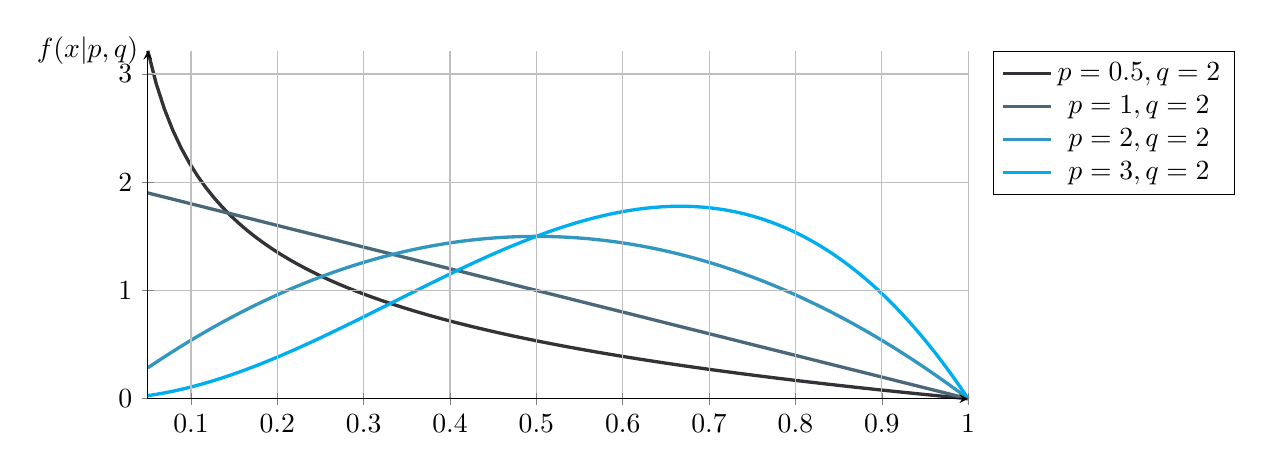
\begin{tikzpicture}[
        declare function={gamma(\z)=
        2.506628274631*sqrt(1/\z)+ 0.20888568*(1/\z)^(1.5)+ 0.00870357*(1/\z)^(2.5)- (174.2106599*(1/\z)^(3.5))/25920- (715.6423511*(1/\z)^(4.5))/1244160)*exp((-ln(1/\z)-1)*\z;},
        declare function={betapdf(\x,\p,\q) = gamma(\p+\q)/(gamma(\p)*gamma(\q)) * \x^(\p-1)*(1-x)^(\q-1);}
        ]
        \begin{axis}[
            ylabel={$f(x | p, q)$},
            domain=0.05:1, samples=100,
            axis lines=left,
            every axis y label/.style={at=(current axis.above origin),anchor=east},
            every axis x label/.style={at=(current axis.right of origin),anchor=north},
            height=6cm, width=12cm,
            enlargelimits=false, clip=false, axis on top,
            grid = major,
            legend pos=outer north east
        ]
            \addplot [very thick,cyan!10!black] {betapdf(x,0.5,2)};
            \addlegendentry{$p = 0.5, q = 2$}
            \addplot [very thick,cyan!40!black] {betapdf(x,1,2)};
            \addlegendentry{$p = 1, q = 2$}
            \addplot [very thick,cyan!75!black] {betapdf(x,2,2)};
            \addlegendentry{$p = 2, q = 2$}
            \addplot [very thick,cyan] {betapdf(x,3,2)};
            \addlegendentry{$p = 3, q = 2$}
        \end{axis}
    \end{tikzpicture}
    \caption{Densidad de la distribución beta con distintos valores de $p$.}
    \label{fig:beta:p}
\end{figure}

\begin{figure}[H]
    \centering
    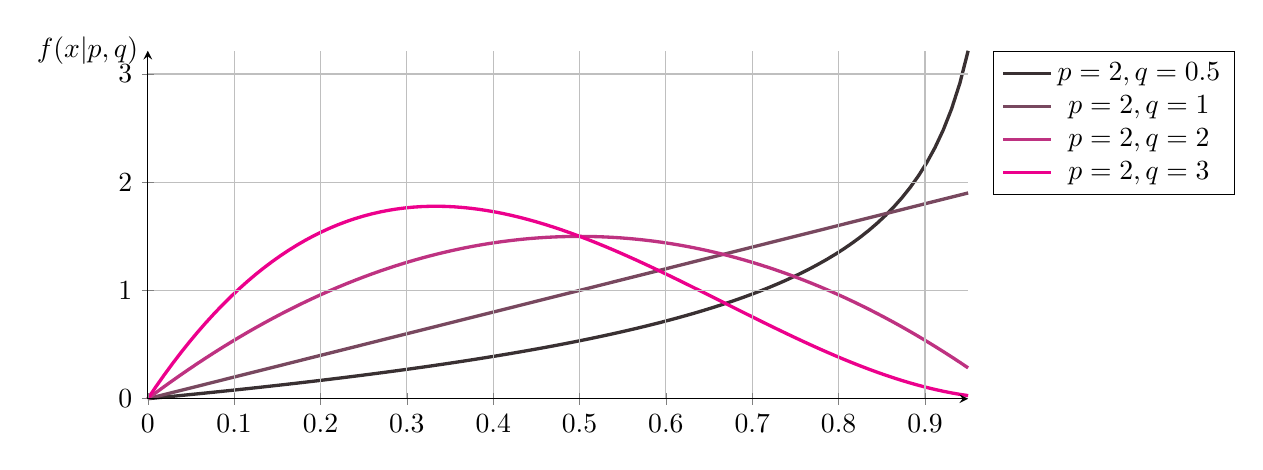
\begin{tikzpicture}[
        declare function={gamma(\z)=
        2.506628274631*sqrt(1/\z)+ 0.20888568*(1/\z)^(1.5)+ 0.00870357*(1/\z)^(2.5)- (174.2106599*(1/\z)^(3.5))/25920- (715.6423511*(1/\z)^(4.5))/1244160)*exp((-ln(1/\z)-1)*\z;},
        declare function={betapdf(\x,\p,\q) = gamma(\p+\q)/(gamma(\p)*gamma(\q)) * \x^(\p-1)*(1-x)^(\q-1);}
        ]
        \begin{axis}[
            ylabel={$f(x | p, q)$},
            domain=0:0.95, samples=100,
            axis lines=left,
            every axis y label/.style={at=(current axis.above origin),anchor=east},
            every axis x label/.style={at=(current axis.right of origin),anchor=north},
            height=6cm, width=12cm,
            enlargelimits=false, clip=false, axis on top,
            grid = major,
            legend pos=outer north east
        ]
            \addplot [very thick,magenta!10!black] {betapdf(x,2,0.5)};
            \addlegendentry{$p = 2, q = 0.5$}
            \addplot [very thick,magenta!40!black] {betapdf(x,2,1)};
            \addlegendentry{$p = 2, q = 1$}
            \addplot [very thick,magenta!75!black] {betapdf(x,2,2)};
            \addlegendentry{$p = 2, q = 2$}
            \addplot [very thick,magenta] {betapdf(x,2,3)};
            \addlegendentry{$p = 2, q = 3$}
        \end{axis}
    \end{tikzpicture}
    \caption{Densidad de la distribución beta con distintos valores de $q$.}
    \label{fig:beta:q}
\end{figure}

\begin{figure}[H]
    \centering
    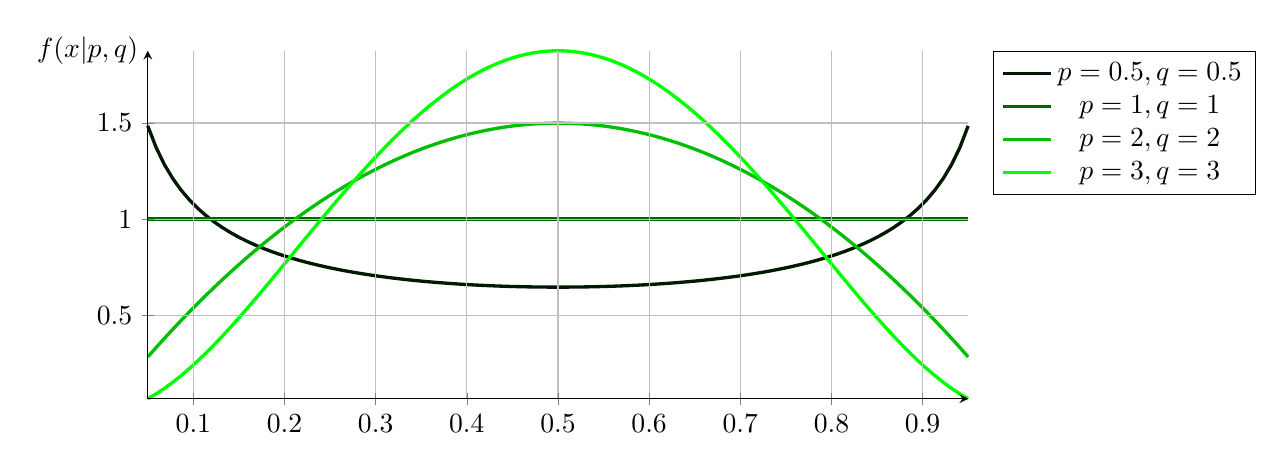
\begin{tikzpicture}[
        declare function={gamma(\z)=
        2.506628274631*sqrt(1/\z)+ 0.20888568*(1/\z)^(1.5)+ 0.00870357*(1/\z)^(2.5)- (174.2106599*(1/\z)^(3.5))/25920- (715.6423511*(1/\z)^(4.5))/1244160)*exp((-ln(1/\z)-1)*\z;},
        declare function={betapdf(\x,\p,\q) = gamma(\p+\q)/(gamma(\p)*gamma(\q)) * \x^(\p-1)*(1-x)^(\q-1);}
        ]
        \begin{axis}[
            ylabel={$f(x | p, q)$},
            domain=0.05:0.95, samples=100,
            axis lines=left,
            every axis y label/.style={at=(current axis.above origin),anchor=east},
            every axis x label/.style={at=(current axis.right of origin),anchor=north},
            height=6cm, width=12cm,
            enlargelimits=false, clip=false, axis on top,
            grid = major,
            legend pos=outer north east
        ]
            \addplot [very thick,green!10!black] {betapdf(x,0.5,0.5)};
            \addlegendentry{$p = 0.5, q = 0.5$}
            \addplot [very thick,green!40!black] {betapdf(x,1,1)};
            \addlegendentry{$p = 1, q = 1$}
            \addplot [very thick,green!75!black] {betapdf(x,2,2)};
            \addlegendentry{$p = 2, q = 2$}
            \addplot [very thick,green] {betapdf(x,3,3)};
            \addlegendentry{$p = 3, q = 3$}
        \end{axis}
    \end{tikzpicture}
    \caption{Densidad de la distribución beta con $p = q$.}
    \label{fig:beta:pq}
\end{figure}

\begin{prop}
    La función característica de la distribución $beta(x|p,q)$ viene dada por
    \[\varphi_X(t) = 1 + \sum_{k = 1}^\infty \frac{(it)^k}{k!} \frac{\beta(p+k,q)}{\beta(p,q)}.\]
\end{prop}

\begin{proof}
Desarrollamos la función característica utilizando el desarrollo de la exponencial
\begin{gather*}
E[e^{itX}] = \frac{1}{\beta(p,q)}\int_0^1 e^{itx} x^{p-1}(1-x)^{q-1} dx = \frac{1}{\beta(p,q)}\int_0^1 \sum_{k = 0}^\infty \frac{(itx)^{k}}{k!} x^{p-1}(1-x)^{q-1} dx \\
= \frac{1}{\beta(p,q)}\sum_{k = 0}^\infty \frac{(it)^k}{k!} \int_0^1x^{p+k-1}(1-x)^{q-1} dx = \sum_{k = 0}^\infty \frac{(it)^k}{k!} \frac{\beta(p+k,q)}{\beta(p,q)} = 1 + \sum_{k = 1}^\infty \frac{(it)^k}{k!} \frac{\beta(p+k,q)}{\beta(p,q)}. \qedhere
\end{gather*}
\end{proof}

\begin{cor} \label{cor:beta:moments}
    Sea $X \sim beta(x|p,q)$. Entonces, para cada $k \ge 1$ se tiene que
    \[E[X^k] = \frac{\beta(p+k,q)}{\beta(p,q)}.\]
\end{cor}

\begin{cor} \label{cor:beta:esp}
    Sea $X \sim beta(x|p,q)$. Entonces, $E[X] = \frac{p}{p+q}$ y $Var(X) = \frac{pq}{(p+q)^2(p+q+1)}$.
\end{cor}
\begin{proof}
    Por el Corolario \ref{cor:beta:moments} y la Proposición \ref{prop:beta-gamma} tenemos que
    \[E[X] = \frac{\beta(p+1,q)}{\beta{p,q}} = \frac{\Gamma(p+1)\Gamma(q)}{\Gamma(p+q)} \frac{\Gamma(p+q)}{\Gamma(p)\Gamma(q)} = \frac{\Gamma(p+1)}{\Gamma(p)} \frac{\Gamma(p+q)}{\Gamma(p+q+1)} = \frac{p}{p+q}\]
    y
    \[E[X^2] = \frac{\beta(p+2,q)}{\beta{p,q}} = \frac{\Gamma(p+2)\Gamma(q)}{\Gamma(p+q+2)} \frac{\Gamma(p+q)}{\Gamma(p)\Gamma(q)} = \frac{\Gamma(p+2)}{\Gamma(p)} \frac{\Gamma(p+q)}{\Gamma(p+q+2)} = \frac{p(p+1)}{(p+q)(p+q+1)}.\]
    Por último, es directo calcular $Var(X) = E[X^2] - E[X]^2$.
\end{proof}

\subsubsection{Distribución de Cauchy}

\begin{definition}
    Sea $\mu \in \mathbb{R}$ y $\sigma > 0$. Definimos la distribución $Cauchy(x | \mu, \sigma)$ como la distribución que tiene función de densidad
    \[f(x | \mu, \sigma) = \frac{1}{\sigma \pi} \frac{1}{1+\left(\frac{x-\mu}{\sigma}\right)^2} = \frac{\sigma}{\pi(\sigma^2 + (x-\mu)^2)}, \ x \in \mathbb{R}.\]
\end{definition}

La distribución está bien definida. En efecto, utilizando el cambio de variable $x = \sigma y + \mu$ obtenemos
\[\int_{-\infty}^\infty \frac{1}{1+\left(\frac{x-\mu}{\sigma}\right)^2} dx = \int_{-\infty}^\infty \frac{\sigma}{1+y^2} dy = \sigma \pi.\]

\begin{prop}
    La función característica de la distribución $Cauchy(x|\mu,\sigma)$ viene dada por
    \[\varphi_X(t) = e^{i\mu t - \sigma |t|}.\]
\end{prop}
\begin{proof}
    En primer lugar, demostramos el resultado para $Cauchy(x|0,1)$. Tenemos que
    \[\varphi_X(t)  = \frac{1}{\pi}\int_{-\infty}^\infty \frac{e^{itz}}{1+z^2} dz = e^{-|t|},\]
    donde la última igualdad se explica en \cite{cauchy}. Ahora, si $X \sim Cauchy(x|\mu,\sigma)$, entonces $Y = (X - \mu) / \sigma \sim Cauchy(x|0,1)$ y, por tanto, obtenmos
    \[\varphi_X(t) = E[e^{itX}] = E[e^{it(\sigma Y+\mu)}] = e^{it\mu} \varphi_Y(\sigma t) = e^{i\mu t - \sigma |t|}. \qedhere\]
\end{proof}

Nótese que la función característica de la distribución de Cauchy no es diferenciable en $0$. Consecuentemente, esta distribución no tiene momentos de orden mayor o igual que 1. El recíproco no sería cierto, esto es, existen distribuciones que no tienen esperanza y su función característica es diferenciable en $0$ \cite{char}.

\begin{prop}
    Sean $X$ e $Y$ dos variables aleatorias independientes con distribuciones $Cauchy(x|\mu_1, \sigma_1)$ y $Cauchy(x|\mu_2, \sigma_2)$ respectivamente. Entonces, $X+Y \sim Cauchy(x|\mu_1+\mu_2,\sigma_1+\sigma_2)$.
\end{prop}
\begin{proof}
    Nótese que $\varphi_{X+Y}(t) = \varphi_{X}(t)\varphi_{Y}(t) = e^{it(\mu_1+\mu_2) - |t| (\sigma_1+\sigma_2)}$. La prueba finaliza al darse cuenta de que ésta es la función característica de $Cauchy(x|\mu_1+\mu_2,\sigma_1+\sigma_2)$.
\end{proof}

\begin{figure}[H]
    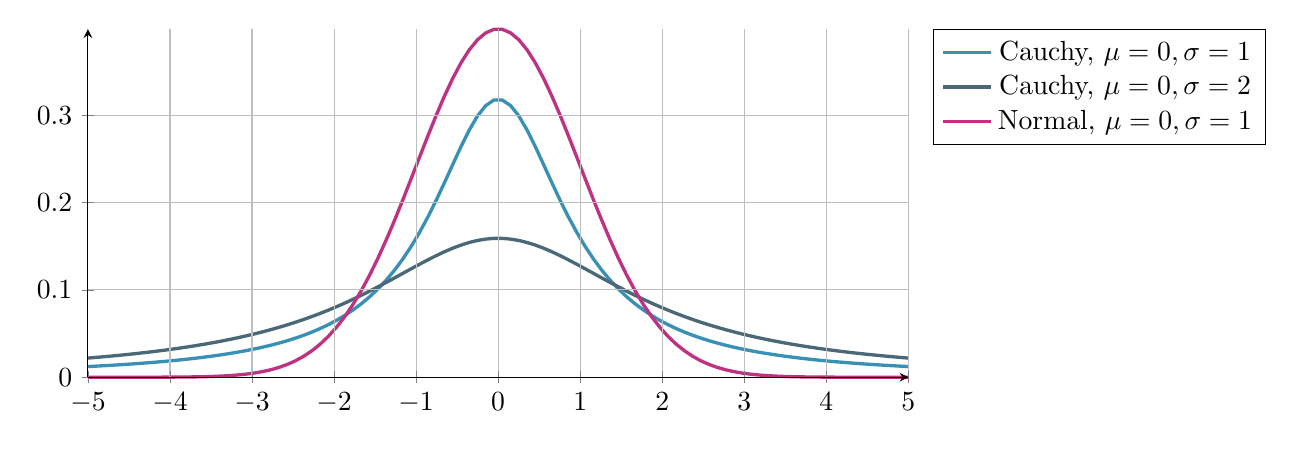
\begin{tikzpicture}[
            declare function={gauss(\x,\mu,\sigma)=1/(\sigma*sqrt(2*pi))*exp(-((\x-\mu)^2)/(2*\sigma^2));},
            declare function={cauchy(\x,\mu,\sigma) = 1/((\sigma*pi)*(1+((\x-\mu)/\sigma)^2));}
        ]
        \begin{axis}[
            domain=-5:5, samples=100,
            axis lines=left,
            every axis y label/.style={at=(current axis.above origin),anchor=east},
            every axis x label/.style={at=(current axis.right of origin),anchor=north},
            height=6cm, width=12cm,
            enlargelimits=false, clip=false, axis on top,
            grid = major,
            legend pos=outer north east
        ]
            \addplot [very thick,cyan!70!black] {cauchy(x,0,1)};
            \addlegendentry{Cauchy, $\mu = 0, \sigma = 1$}
            \addplot [very thick,cyan!40!black] {cauchy(x,0,2)};
            \addlegendentry{Cauchy, $\mu = 0, \sigma = 2$}
            \addplot [very thick,magenta!75!black] {gauss(x,0,1)};
            \addlegendentry{Normal, $\mu = 0, \sigma = 1$}
        \end{axis}
    \end{tikzpicture}
    \caption{Densidad de la distribución de Cauchy comparada con la distribución normal.}
    \label{fig:cauchy}
\end{figure}


\subsubsection{Distribución de Laplace}

\begin{definition}
    Sea $\mu \in \mathbb{R}$ y $\sigma > 0$. Definimos la distribución de Laplace, y la denotamos $Laplace(x | \mu, \sigma)$ como la distribución que tiene función de densidad
    \[f(x | \mu, \sigma) = \frac{1}{2 \sigma} e^{-|x - \mu| / \sigma}, \ x \in \mathbb{R}.\]
\end{definition}

\begin{figure}[H]
    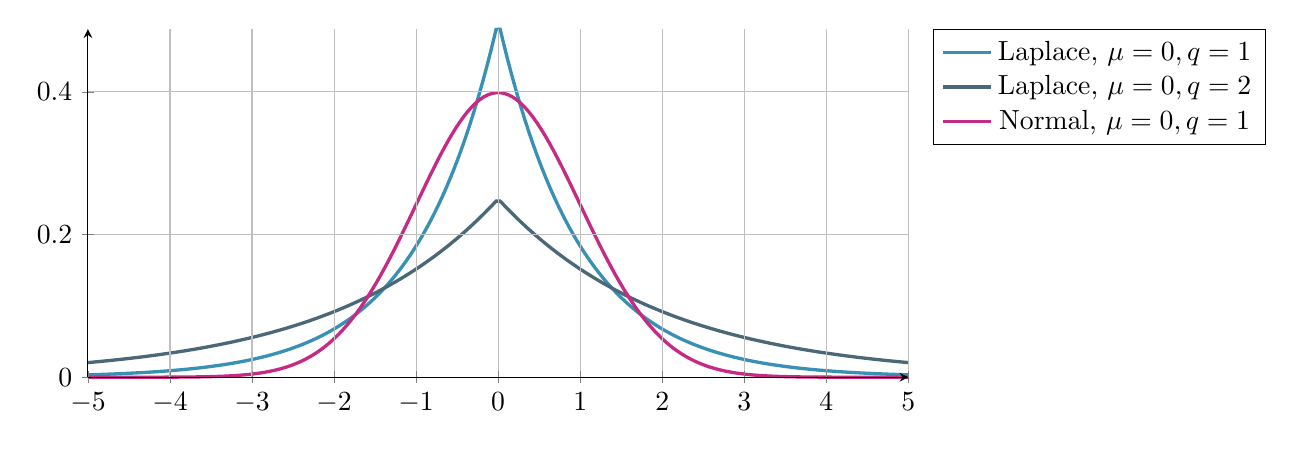
\begin{tikzpicture}[
         declare function={gauss(\x,\mu,\sigma)=1/(\sigma*sqrt(2*pi))*exp(-((\x-\mu)^2)/(2*\sigma^2));},
         declare function={laplace(\x,\mu,\sigma) = exp(-abs(\x-\mu) / \sigma)/(2*\sigma);}
        ]
        \begin{axis}[
            domain=-5:5,
            samples=200,
            axis lines=left,
            every axis y label/.style={at=(current axis.above origin),anchor=east},
            every axis x label/.style={at=(current axis.right of origin),anchor=north},
            height=6cm, width=12cm,
            enlargelimits=false,
            clip=false,
            axis on top,
            grid = major,
            legend pos=outer north east
        ]
            \addplot [very thick,cyan!70!black] {laplace(x,0,1)};
            \addlegendentry{Laplace, $\mu = 0, q = 1$}
            \addplot [very thick,cyan!40!black] {laplace(x,0,2)};
            \addlegendentry{Laplace, $\mu = 0, q = 2$}
            \addplot [very thick,magenta!80!black] {gauss(x,0,1)};
            \addlegendentry{Normal, $\mu = 0, q = 1$}
        \end{axis}
    \end{tikzpicture}
    \caption{Densidad de la distribución de Laplace comparada con la densidad de la distribución normal.}
    \label{fig:laplace}
\end{figure}


\subsubsection{Distribución T de Student}

\subsubsection{Distribución de Dirichlet}
		La distribución de Dirichlet es la generalización en multivariable de la distribución Beta. Comúnmente, se utilizan las funciones de Dirichlet como funciones a priori en estadística Bayesiana. Definimos la distribución de Dirichlet de orden $n \geq 2$ con parámetros $\alpha_1, ..., \alpha_n$ tiene una función de densidad de probabilidad

		\begin{equation*}
		f(x_1, .. x_n|\alpha_1, ...,\alpha_n) = \frac{\Gamma(\alpha_1 + ... + \alpha_n)}{\Gamma(\alpha_1) + ... + \Gamma(\alpha_n)} \prod_{i=1}^{n} {x_i ^ {\alpha_i - 1}}
		\end{equation*}

		definida en el simplex abierto de (n-1) dimensiones definido por:

		\begin{equation*}
		x_1, ... , x_n > 0
		\end{equation*}
		\begin{equation*}
		x_1 + ... + x_{n-1} < 1
		\end{equation*}
		\begin{equation*}
		x_n =  1 - x_1 - ... - x_{n-1}
		\end{equation*}

		\begin{thm}
			Sea $X = (X_1, ... , X_k) \sim Dirichlet(X|\alpha_1, ... , \alpha_k, \alpha_{k+1}) $ se tiene que para cualquier $k_1 < k$  se verifica que $X' =  (X_1, ... , X_{k_1}) \sim D(X'|\alpha_1, ... , \alpha_{k_1}, \alpha_{k_1 + 1}^{*}) $ con  $\alpha_{k+1}^{*} =\sum_{j=1}^{k_1} {\alpha_{j}}$
		\end{thm}

		\begin{proof}
			Pendiente
		\end{proof}
